\chapter{Potências e funções exponenciais}

\section{Introdução}

As funções exponenciais modelam uma série de problemas de interesse científico tais como aplicações financeiras a juros compostos, crescimento populacional, reações químicas, secagem de produtos agrícolas, entre outras.

\section{Potências}

\begin{caixa}
\textbf{Definição 2.1: }A potência \textit{n $ \epsilon $  Z}  , \textit{n > 0}, de um número \textit{b $ \epsilon $   } é o produto de \textit{b}, \textit{n} vezes, por ele mesmo:

\begin{figure}[H]
	\begin{Center}
		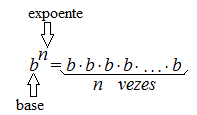
\includegraphics[width=2.05in,height=1.2in]{capitulos/potencias_e_funcoes_exponenciais/media/image2.png}
	\end{Center}
\end{figure}
\end{caixa}

\begin{texemplo}
Calcule  (a) \textit{2\textsuperscript{3}} , (b) (-3)\textit{\textsuperscript{4} ,} (c) \textit{-3\textsuperscript{4}}e  (d)  \(  \left( \frac{1}{2} \right) ^{3} \) 

\textbf{Solução}: 

(a) \textit{2\textsuperscript{3}}= 2 $ \cdot $  2 $ \cdot $  2  = \textit{8}

(b) (-3)\textit{\textsuperscript{4} = (-3)} $ \cdot $  \textit{(-3)} $ \cdot $  \textit{(-3)} $ \cdot $  \textit{(-3)} = \textit{81 }

(c) \textit{-3\textsuperscript{4} = - 3} $ \cdot $  \textit{3} $ \cdot $  \textit{3} $ \cdot $ \textit{3 = -81}

(d)  \(  \left( \frac{1}{2} \right) ^{3}=\frac{1}{2}  \cdot \frac{1}{2} \cdot \frac{1}{2}=\frac{1}{8} \) 
\end{texemplo}

\textbf{Propriedade das potências}

\begin{caixa}
\textbf{P1}: $b^n \cdot b^m = b^{n+m}$ (\textbf{Produto de potências de mesma base})
\end{caixa}

\textbf{Demonstração}: Expandindo as potências, temos o produto de \textit{n} bases \textit{b} por \textit{m} bases \textit{b}. Como todas as bases são iguais, pela Def. 2.1, o expoente será \textit{n + m}.

\begin{figure}[H]
	\begin{Center}
		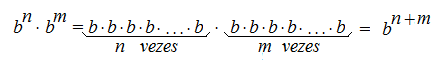
\includegraphics[width=4.61in,height=0.64in]{capitulos/potencias_e_funcoes_exponenciais/media/image3.png}
	\end{Center}
\end{figure}

\qedsymbol{}

\begin{texemplo}
Resolva os produtos de potências: 

 (a)  \textit{2\textsuperscript{3}} $ \cdot $  \textit{2\textsuperscript{5}}   e   (b)  \(  \left( \frac{2}{3} \right) ^{2} \cdot  \left( \frac{2}{3} \right) ^{3} \) .

\textbf{Solução}: 

(a) \textit{2\textsuperscript{3}}$ \cdot $   \textit{2\textsuperscript{5}} = \textit{2\textsuperscript{3+5}} = \textit{2\textsuperscript{8}} 

(b)  \(  \left( \frac{2}{3} \right) ^{2} \cdot  \left( \frac{2}{3} \right) ^{3}= \left( \frac{2}{3} \right) ^{2+3}= \left( \frac{2}{3} \right) ^{5} \)  \qedsymbol{}
\end{texemplo}

\begin{caixa}
\textbf{P2}: \( \frac{b^{m}}{b^{n}}=b^{m}: b^{n}=b^{m-n} \). (\textbf{Divisão de potências de mesma base})
\end{caixa}

\textbf{Demonstração}: Escrevendo a divisão como fração e expandindo as potências, podemos cancelar as bases \textit{b} do numerador e denominador. O número de bases restantes será \textit{n - m}.

\begin{figure}[H]
			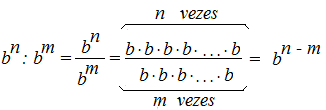
\includegraphics[width=3.4in,height=1.15in]{capitulos/potencias_e_funcoes_exponenciais/media/image4.png}
	\end{figure}

\qedsymbol{}

\begin{texemplo}
Resolva as divisões de potências: 

  (a) 3\textit{\textsuperscript{4}} : \textit{3\textsuperscript{2}}   e   (b)  \(  \left( \frac{5}{2} \right) ^{5} \cdot  \left( \frac{5}{2} \right) ^{3} \) .

\textbf{Solução}: 

 (a) \textit{3\textsuperscript{4}} : \textit{3\textsuperscript{2}} = \textit{3\textsuperscript{4-2}} = \textit{3\textsuperscript{2}}  

 (b)  \(  \left( \frac{5}{2} \right) ^{5} \cdot  \left( \frac{5}{2} \right) ^{3}= \) . \(  \left( \frac{5}{2} \right) ^{5-3}= \left( \frac{5}{2} \right) ^{2} \)  \qedsymbol{}
\end{texemplo}

\begin{caixa}
\textbf{P3}: $b^0 = 1$. (\textbf{Expoente zero})
\end{caixa}

\textbf{Demonstração}: Seja  \( \frac{b^{n}}{b^{n}}=1 \) .Pela P2, tem-se   \( \frac{b^{n}}{b^{n}}=b^{n-n}=b^{0}=1 \)  \qedsymbol{}

\begin{texemplo}
    (a)Mostre que :   3\textit{\textsuperscript{4}} : \textit{3\textsuperscript{4}} = 1. 

    (b) Resolva a expressão numérica:  \(  \left(  \left( \frac{3}{2} \right) ^{0}+\frac{1}{2} \right) ~  \cdot  \left( \frac{3}{2} \right) ^{2} \) .

\textbf{Solução}: 

 (a) \textit{3\textsuperscript{4}} : \textit{3\textsuperscript{4}} = \textit{3\textsuperscript{4-4}} = \textit{3\textsuperscript{0}} = 1  

 (b)  \(  \left(  \left( \frac{3}{2} \right) ^{0}+\frac{1}{2} \right) ~  \cdot  \left( \frac{3}{2} \right) ^{2}= \left( 1+\frac{1}{2} \right) ~  \cdot  \left( \frac{3}{2} \right) ^{2}= \left( \frac{3}{2} \right) ~  \cdot  \left( \frac{3}{2} \right) ^{2}= \left( \frac{3}{2} \right) ^{3} \)  \qedsymbol{}
\end{texemplo}

\begin{caixa}
\textbf{P4}:  \( b^{-n}= \frac{1}{b^{n}} \)  \textit{. }(\textbf{Expoente negativo})
\end{caixa}

\textbf{Demonstração}: Sejam \textit{b\textsuperscript{p} }e  \textit{b\textsuperscript{q}} , tal que  \textit{n = q - p > 0}. Usando a P2, tem-se:

   \( b^{-n}=b^{p-q}=\frac{b^{p}}{b^{q}} \)  . Expandindo as potências e cancelando as bases \textit{b}, o numerador será \textit{1} e o denominador terá \textit{n = q - p} bases \textit{b}. Então,

 \( b^{-n}= \frac{1}{b^{n}} \) . \qedsymbol{}

\begin{texemplo}
    (a)Mostre que :    \(  \left( \frac{a}{b} \right) ^{-1}=\frac{b}{a} \) . 

   (b) Resolva a expressão n umérica:  \(  \left(  \left( \frac{1}{3} \right) ^{-1}+2 \right) ^{-2} \) .

\textbf{Solução}: 

 (a)Usando a P4:   \(  \left( \frac{a}{b} \right) ^{-1}=\frac{1}{\frac{a}{b}}=1 \cdot \frac{b}{a}=\frac{b}{a} \)  .

 (b)Resolvendoinicialmente dentro do parênteses da potência maior, aplicando a P4:   

  \(   \left(  \left( \frac{1}{3} \right) ^{-1}+2 \right) ^{-2}= \left( 3+2 \right) ^{-2}=5^{-2} \)  . Aplicando a P4, novamente:

  \( 5^{-2}=\frac{1}{5^{2}}=\frac{1}{25} \)   \qedsymbol{}
\end{texemplo}

\begin{caixa}
\begin{figure}[H]
    \begin{Center}
        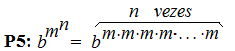
\includegraphics[width=2.45in,height=0.53in]{capitulos/potencias_e_funcoes_exponenciais/media/image5.png}
        (\textbf{Potência de expoente})
	\end{Center}
\end{figure}
\end{caixa}

\textbf{Demonstração}: Expandindo a potência \textit{m\textsuperscript{n}} obtém-se o expoente de  \( b^{m^{n}} \)  \qedsymbol{}

\begin{texemplo}
Resolva: (a)  \( 2^{2^{3}} \)  (b)  $2^{(-3)^{2}}$.

\textbf{Solução}: 

 (a) Usando a P5:  \( 2^{2 \cdot 2 \cdot 2}=2^{8}=256. \)  .

 (b) Usandoa P5:   \( 2^{ \left( -3 \right)  \cdot  \left( -3 \right) }=2^{9} \)  \qedsymbol{}
\end{texemplo}

\begin{caixa}
\textbf{P6:} $(b^m)^n = b^{m \cdot n}$ (\textbf{Potência de potência})
\end{caixa}

\textbf{Demonstração}: Expandindo a potência \textit{(b\textsuperscript{m})\textsuperscript{n}} obtém-se um produto de \textit{n} fatores, cuja base é \textit{b}. Usando a propriedade do produto (P1), conserva-se a base e soma-se os \textit{n} expoentes \textit{m}. Então,

\begin{figure}[H]
	\begin{Center}
		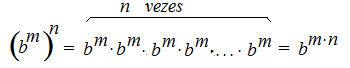
\includegraphics[width=3.65in,height=0.71in]{capitulos/potencias_e_funcoes_exponenciais/media/image6.png}
	\end{Center}
\end{figure}

 \qedsymbol{}

\begin{texemplo}
Resolva: (a) \(  \left(  \left( -2 \right) ^{2} \right) ^{3} \)  (b)  \(  \left( 2^{ \left( -3 \right) } \right) ^{2} \) .

\textbf{Solução}: 

(a) Usandoa P6:   \(  \left(  \left( -2 \right) ^{2} \right) ^{3}= \left( -2 \right) ^{2 \cdot 3}= \left( -2 \right) ^{6}=64~  \)  

ou usando a Def. 2.1:

  \(  \left(  \left( -2 \right) ^{2} \right) ^{3}= \left( -2 \right) ^{2} \cdot  \left( -2 \right) ^{2} \cdot  \left( -2 \right) ^{2}= \left( -2 \right) ^{6}=64  \)  .

 (b)Usando a P6:   \(  \left( 2^{ \left( -3 \right) } \right) ^{2}=2^{-6}=\frac{1}{2^{6}} \)  \qedsymbol{}
\end{texemplo}

\begin{caixa}
\textbf{P7}:  \(  \left( \frac{a}{b} \right) ^{n}=\frac{a^{n}}{b^{n}} \)  (\textbf{Potência de fração})
\end{caixa}

A demonstração desta propriedade é obtida diretamente com a Def. 2.1. 

\begin{texemplo}Resolva:(a)   \(  \left( \frac{2}{3} \right) ^{3} \)  (b)  \(  \left( -\frac{3}{4} \right) ^{-2} \) .

\textbf{Solução}: 

 (a)Usando a P7:   \(  \left( \frac{2}{3} \right) ^{3}=\frac{2^{3}}{3^{3}}=\frac{8}{27} \)  .

 (b)Usandoa P4:    \(  \left( -\frac{3}{4} \right) ^{-2}= \left( -\frac{4}{3} \right) ^{2}. \)  Usando a P7:   \(  \left( -\frac{4}{3} \right) ^{2}=\frac{16}{9}. \)  \qedsymbol{}
\end{texemplo}

\begin{caixa}
\textbf{P8}:  \(  \left( a \cdot b \right) ^{n}=a^{n} \cdot b^{n} \)  (\textbf{Potência do produto})
\end{caixa}

\textbf{Demonstração}: Expandindo a base (a b) n vezes e usando a Def. 2.1 para os fatores \textit{a} e \textit{b}, obtem-se o produto de \textit{a\textsuperscript{n} . b\textsuperscript{n}}.

\begin{figure}[H]
	\begin{Center}
		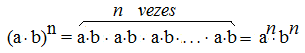
\includegraphics[width=3.18in,height=0.55in]{capitulos/potencias_e_funcoes_exponenciais/media/image7.png}
	\end{Center}
\end{figure}

\qedsymbol{}

\begin{texemplo}
Resolva:(a)   \(  \left( 2 \cdot 3 \right) ^{3} \)  (b) \(   \left( 2+3 \right) ^{3} \) .

\textbf{Solução}: 

 (a) Usando a P8:  \( 2^{3} \cdot 3^{3}=8  \cdot 27=216. \)  .

 (b) Nessecaso não é possível aplicar a P8, mas pode-se adicionar dentro do parênteses e aplicar a definição:   \(  \left( 2+3 \right) ^{3}=5^{3}=125 \)  \qedsymbol{}
\end{texemplo}

\begin{caixa}
\textbf{P9}. Se \textit{b\textsuperscript{m} = b\textsuperscript{n}} então \textit{m = n}. (\textbf{Igualdade de duas potências: bases iguais})
\end{caixa}

\textbf{Demonstração: }Dividindo \textit{b\textsuperscript{m} = b\textsuperscript{n} por b\textsuperscript{m} , }obtem-se

  \( 1=\frac{b^{n}}{b^{m}}= b^{m-n} \) .Portanto,pela propriedade do expoente zero (P3) tem-se   \textit{m - n = 0} ou \textit{m = n} \qedsymbol{}

\begin{texemplo}
Resolva as equações exponenciais: 

 (a)  \( 2^{x}= \left( \frac{1}{2} \right) ^{-1} \)  (b) \(  7^{2x+1}=\frac{1}{49} \) .

\textbf{Solução}: 

 (a) Para usar a P9, é necessário que as bases das potências sejam iguais.  Usando a P4 no lado direito:  \( 2^{x}= \left( \frac{1}{2} \right) ^{-1}=2 \) . Usando a P9: \textit{x = 1}.

 (b) Para usar a P9, é necessário que as bases das potências sejam iguais.  Decompondo o 49 e usando a P4 no lado direito:  \( 7^{2x+1}=7^{-2} \)  . Usando a  P9:   \( 2x+1=-2 \)  . resolvendo para \textit{x}tem-se:  \textit{x = -3/2} \qedsymbol{}
\end{texemplo}

\textbf{P10}. (\textbf{Igualdade de duas potências: expoentes iguais})

 Se \textit{a\textsuperscript{m} = b\textsuperscript{m}} , para \textit{m $ \neq $  0}, \textit{a,} \textit{b} e \textit{m} $ \epsilon $  , então \textit{a = b}.

\textbf{Demonstração}: Dividindo \textit{a\textsuperscript{m} = b\textsuperscript{m}} por \textit{ a\textsuperscript{m}  }e usando as propriedades P3 e P7, obtém-se

  \( 1=\frac{b^{m}}{a^{m}}=  \left( \frac{b}{a} \right) ^{m} \) . Como \textit{m $ \neq $  0}, para que essa igualdade seja verdadeira  \( \frac{b}{a}=1 \) ou  \textit{a = b} \qedsymbol{}

\begin{texemplo}
Resolva a equação exponencial:   \( 16= \left( 3x-2 \right) ^{4} \) .

\textbf{Solução}: 

 Para usar a P10, é necessário que os expoentes das potências sejam iguais.  Decompondo 16, tem-se :  \( 2^{4}= \left( 3x-2 \right) ^{4} \) . Usando a P10:

  \( 2=3x-2  \) . Resolvendo para \textit{x}, tem-se \textit{x = 4/3} \qedsymbol{}
\end{texemplo}

\begin{exercicios}
\exitem{} Calcule as potências:

\begin{multicols}{4}
    a) \textit{4\textsuperscript{2}} =
    
    b) (-4)\textsuperscript{3}=

    c) 0\textsuperscript{5} =

    d) 1\textsuperscript{100} =

    e)  \(  \left( \frac{1}{2} \right) ^{3}= \)
    
    f)  \(  \left( -\frac{3}{4} \right) ^{2}= \)

    g)  \(  \left( \frac{2}{3} \right) ^{4}= \) 
    
    h)  \( -5^{4}= \) 
\end{multicols}

\exitem{} Resolva as operações com as potências usando as propriedades P1 e P2:

\begin{multicols}{4}
a)  \textit{2\textsuperscript{2} $ \cdot $} \textit{2\textsuperscript{4} =}

b) $\left(\frac{1}{2}\right) ^{3} \cdot  \left( \frac{1}{2} \right) ^{2} \cdot  \left( \frac{1}{2} \right) ^{5}=$

c) \textit{3\textsuperscript{4} :} \textit{3\textsuperscript{2} =}

d)  \(  \left( \frac{3}{2} \right) ^{4} \cdot  \left( \frac{3}{2} \right) ^{2}= \)

e)  \(  \left( \frac{5}{4} \right) ^{3}: \left( \frac{5}{4} \right) ^{2}= \)

f) \textit{5\textsuperscript{2} :} \textit{5\textsuperscript{5} =}

g)  \(  \left( \frac{7}{4} \right) ^{3}: \left( \frac{7}{4} \right) ^{5}= \)  

h) \textit{8\textsuperscript{-2} $ \cdot $ } \textit{8\textsuperscript{5 }=}
\end{multicols}

\exitem{} Resolva as potências usando a propriedade do expoente negativo:

a)  \textit{2\textsuperscript{-3} = } b) \textit{3\textsuperscript{-5}  =} c)  \(  \left( \frac{3}{4} \right) ^{-3}= \)   d)  \(  \left( \frac{3}{4} \right) ^{-2}= \)  

\item Mostre que  \(  \left( \frac{a}{b} \right) ^{-n}= \left( \frac{b}{a} \right) ^{n} \) .

\item Verifique se  \( 2^{3^{2}}=  \left( 2^{3} \right) ^{2} \) .

\exitem{} Resolva as expressões numéricas usando as propriedades:

\begin{multicols}{3}
    a)  \(  \left( \frac{2}{5} \right) ^{2} \cdot  \left( \frac{1}{2} \right) ^{-3}= \)
    
    b)  \(  \left( -2 \right) ^{3} \cdot  \left( \frac{3}{2} \right) ^{2} \cdot  \left( \frac{3}{2} \right) ^{-3}=  \)
    
    c)  \(  \left[ 2^{3} \cdot  \left( \frac{1}{2} \right) ^{2} \right] ^{3}= \)

    d)  \(  \left[  \left( \frac{7}{3} \right) ^{2} \cdot 14^{-3} \right] ^{-1}= \)

    e)  \(  \left( \frac{3}{4} \right) ^{3} \cdot  \left( \frac{3}{2} \right) ^{-1}= \) 
    
    f)  \(  \left( -\frac{6}{5} \right) ^{-3} \cdot  \left( \frac{3}{25} \right) ^{-2}= \) 
\end{multicols}

\exitem{} Calcule o valor das expressões:

\begin{multicols}{2}
    a) \( \frac{2- \left( \frac{1}{5}+\frac{3}{10}~  \right)  }{ \left( \frac{5}{2}^{2}- \left( \frac{5}{2} \right) ^{2} \right)  \cdot  \left( \frac{5}{2} \right) ^{-1}}= \)

    b) \(  \left( 7^{\frac{1}{3}} \cdot 7^{-\frac{2}{3}} \cdot  7^{\frac{4}{3}} \right) ^{-2}= \)

    c)  \( 1,333 \ldots + \left( \frac{3}{2} \right) ^{-1}= \) 
    
    d)  \(  \left( \frac{7}{5} \cdot  \left( \frac{49}{25} \right) ^{-1} \cdot 5^{-1}  \cdot  \left( \frac{1}{7} \right) ^{-1} \right) ^{100}= \) 
\end{multicols}

\exitem{} Resolva as equações exponenciais usando as propriedades P9 e P10:

\begin{multicols}{3}
a)  \( 7^{x}=343 \)

b)   \( 4^{x-2}=\frac{1}{2} \)

c)  \(  \left( \frac{1}{25} \right) ^{x}=125 \)

d)  \(  \left( \frac{3}{4} \right) ^{x}=0,75 \)

e)  \(  \left( \frac{4}{25} \right) ^{3x+1}= \left( \frac{5}{2} \right) ^{-x} \) 

f)  \(  \left( \frac{3}{2} \right) ^{x-1}=1 \) 
\end{multicols}

\exitem{} Resolva a equação exponencial:  \(  \left( 243 \right) ^{2x+8/5}= \left[  \left( \frac{1}{3} \right) ^{x} \right] ^{x-1} \) .
\end{exercicios}

\section{Funções exponenciais}

\begin{caixa}
\textbf{Definição:} Uma função exponencial tem a forma

  \textit{f(x) = A$ \cdot $  b \textsuperscript{m $ \cdot $  x      }} (3.1)

onde os parâmetros  \textit{A }e \textit{m} $\in \mathbb{R}$  e a base \textit{b} $ \in \mathbb{R} \textsuperscript{+}$, com \textit{b $ \neq $  1}.
\end{caixa}

\begin{texemplo}
Dadas asfunções   \textit{f(x) =  2\textsuperscript{ x}} e \textit{g(x) =  2\textsuperscript{ - x}} :

\begin{enumerate}
	\item Construa uma tabela com valores de \textit{x, } \textit{f(x)} e \textit{g(x)}.

	\item Faça o gráfico das funções  \textit{f(x)} e \textit{g(x)}.

	\item Verifique se são crescentes ou decrescentes.

	\item Determine o domínio e a imagem das funções.
\end{enumerate}

\textbf{Solução}: Os parâmetros da função \textit{f(x)} são: \textit{A = 1} e \textit{m = 1}. Da função g(x) são \textit{A = 1} e \textit{m = -1.}

(a) atribuindo valores para \textit{x}, calcula-se os valores de \textit{f(x)} e \textit{g(x)}, mostrados na tabela. 

\begin{table}[H]
 			\centering
\begin{tabular}{p{0.58in}p{0.58in}p{0.58in}}
\hline
%row no:1
\multicolumn{1}{|p{0.58in}}{\Centering x} & 
\multicolumn{1}{|p{0.58in}}{\Centering f(x)} & 
\multicolumn{1}{|p{0.58in}|}{\Centering g(x)} \\
\hhline{---}
%row no:2
\multicolumn{1}{|p{0.58in}}{\Centering -3} & 
\multicolumn{1}{|p{0.58in}}{\Centering 0,125} & 
\multicolumn{1}{|p{0.58in}|}{\Centering 8} \\
\hhline{---}
%row no:3
\multicolumn{1}{|p{0.58in}}{\Centering -2} & 
\multicolumn{1}{|p{0.58in}}{\Centering 0,25} & 
\multicolumn{1}{|p{0.58in}|}{\Centering 4} \\
\hhline{---}
%row no:4
\multicolumn{1}{|p{0.58in}}{\Centering -1} & 
\multicolumn{1}{|p{0.58in}}{\Centering 0,5} & 
\multicolumn{1}{|p{0.58in}|}{\Centering 2} \\
\hhline{---}
%row no:5
\multicolumn{1}{|p{0.58in}}{\Centering 0} & 
\multicolumn{1}{|p{0.58in}}{\Centering 1} & 
\multicolumn{1}{|p{0.58in}|}{\Centering 1} \\
\hhline{---}
%row no:6
\multicolumn{1}{|p{0.58in}}{\Centering 1} & 
\multicolumn{1}{|p{0.58in}}{\Centering 2} & 
\multicolumn{1}{|p{0.58in}|}{\Centering 0,5} \\
\hhline{---}
%row no:7
\multicolumn{1}{|p{0.58in}}{\Centering 2} & 
\multicolumn{1}{|p{0.58in}}{\Centering 4} & 
\multicolumn{1}{|p{0.58in}|}{\Centering 0,25} \\
\hhline{---}
%row no:8
\multicolumn{1}{|p{0.58in}}{\Centering 3} & 
\multicolumn{1}{|p{0.58in}}{\Centering 8} & 
\multicolumn{1}{|p{0.58in}|}{\Centering 0,125} \\
\hhline{---}
%row no:9
\multicolumn{1}{|p{0.58in}}{\Centering 4} & 
\multicolumn{1}{|p{0.58in}}{\Centering 16} & 
\multicolumn{1}{|p{0.58in}|}{\Centering 0,0625} \\
\hhline{---}

\end{tabular}
 \end{table}

\begin{figure}[H]
    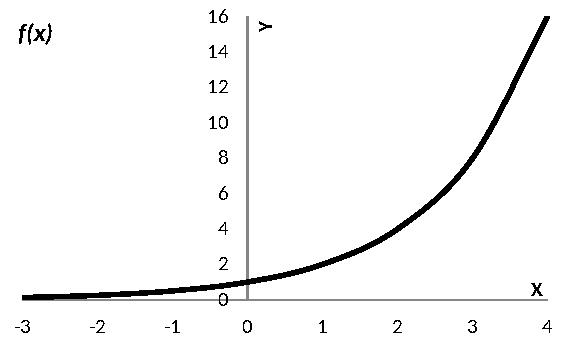
\includegraphics[width=0.45\textwidth]{capitulos/potencias_e_funcoes_exponenciais/media/image8.pdf} 
    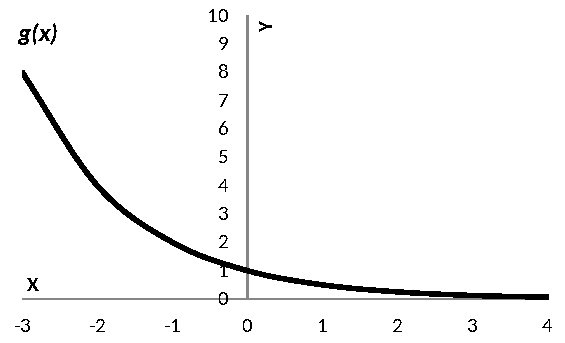
\includegraphics[width=0.45\textwidth]{capitulos/potencias_e_funcoes_exponenciais/media/image9.pdf}
\end{figure}

	\item A função \textit{f(x)} é crescente (sinal do expoente \textit{m} é positivo) e a \textit{g(x)} é decrescente (sinal do expoente \textit{m} é negativo). 

	\item $D_{m} f(x) = \{ x  \in \mathbb{R} \}$ e $I_{m} f(x) = \{x \in \mathbb{R}^{+} \}$

 	\item $D_(m) g(x) = \{ x \in \mathbb{R} \}$ e $I_(m) g(x) = \{x \in \mathbb{R}^{+} \}$

Deve-se observar que a função exponencial é uma função \textit{monótona}: ou cresce, ou decresce, sem apresentar pontos de máximo ou de mínimo como as parábolas, por exemplo. \qedsymbol{}
\end{texemplo}

\begin{texemplo}
As bactérias se reproduzem de forma assexuada, por bipartição. Isto significa que cada indivíduo se parte em dois geneticamente iguais. Em condições favoráveis, se reproduzem rapidamente. Consideremos que uma bactéria se divide a cada \textit{1 h}. Qual será a população de bactérias em 24 h?

\textbf{Solução:} As duas primeiras colunas da tabela abaixo mostram valores das variáveis tempo (\textit{t}) e número de indivíduos (\textit{N}). A terceira coluna mostra expressões numéricas que geram os valores da função \textit{N(t)}.

\begin{table}[H]
 			\centering
\begin{tabular}{p{0.69in}p{0.39in}p{0.69in}}
\hline
%row no:1
\multicolumn{1}{|p{0.69in}}{\Centering Tempo (t)} & 
\multicolumn{1}{|p{0.39in}}{\Centering N(t)} & 
\multicolumn{1}{|p{0.69in}|}{\Centering Expressão} \\
\hhline{---}
%row no:2
\multicolumn{1}{|p{0.69in}}{\Centering 0} & 
\multicolumn{1}{|p{0.39in}}{\Centering 1} & 
\multicolumn{1}{|p{0.69in}|}{\Centering 2\textsuperscript{0}} \\
\hhline{---}
%row no:3
\multicolumn{1}{|p{0.69in}}{\Centering 1} & 
\multicolumn{1}{|p{0.39in}}{\Centering 2} & 
\multicolumn{1}{|p{0.69in}|}{\Centering 2\textsuperscript{1}} \\
\hhline{---}
%row no:4
\multicolumn{1}{|p{0.69in}}{\Centering 2} & 
\multicolumn{1}{|p{0.39in}}{\Centering 4} & 
\multicolumn{1}{|p{0.69in}|}{\Centering 2\textsuperscript{2}} \\
\hhline{---}
%row no:5
\multicolumn{1}{|p{0.69in}}{\Centering 3} & 
\multicolumn{1}{|p{0.39in}}{\Centering 8} & 
\multicolumn{1}{|p{0.69in}|}{\Centering 2\textsuperscript{3}} \\
\hhline{---}
%row no:6
\multicolumn{1}{|p{0.69in}}{\Centering 4} & 
\multicolumn{1}{|p{0.39in}}{\Centering 16} & 
\multicolumn{1}{|p{0.69in}|}{\Centering 2\textsuperscript{4}} \\
\hhline{---}
%row no:7
\multicolumn{1}{|p{0.69in}}{\Centering 5} & 
\multicolumn{1}{|p{0.39in}}{\Centering 32} & 
\multicolumn{1}{|p{0.69in}|}{\Centering 2\textsuperscript{5}} \\
\hhline{---}
%row no:8
\multicolumn{1}{|p{0.69in}}{\Centering ...} & 
\multicolumn{1}{|p{0.39in}}{\Centering ...} & 
\multicolumn{1}{|p{0.69in}|}{\Centering ...} \\
\hhline{---}
%row no:9
\multicolumn{1}{|p{0.69in}}{\Centering t} & 
\multicolumn{1}{|p{0.39in}}{} & 
\multicolumn{1}{|p{0.69in}|}{\Centering 2\textsuperscript{t}} \\
\hhline{---}

\end{tabular}
 \end{table}

Com base na sequência de terceira coluna, as variáveis \textit{N} e \textit{t} se relacionam de acordo com a função \textit{N(t) =  2\textsuperscript{ t}} . Assim, para \textit{t =24}, tem-se \textit{N(24) =  2\textsuperscript{ 24}} , ou seja \textit{N(24)= 16.777.216 }de bactérias \qedsymbol{}
\end{texemplo}

\begin{texemplo}
Faça os gráficos das funções   \( f \left( x \right) = \left( \frac{1}{2} \right) ^{x} \) e  \textit{g(x) = 2\textsuperscript{-x+1}}.

\textbf{Solução:} Usando as propriedades das potências, a \textit{f(x)}pode ser escrita como  

  \( f \left( x \right) = \left( 2^{-1} \right) ^{x}=2^{-x}. \) 

Da mesma forma, \textit{g(x)} pode ser escrita como $g(x) = 2^{-x} \cdot 2^{1}=2 \cdot 2^{-x}$. 

\begin{figure}[H]
	\begin{Center}
		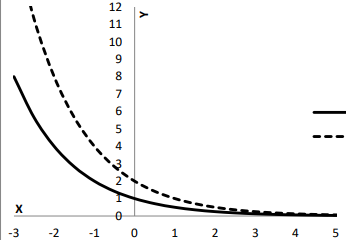
\includegraphics[width=3.62in,height=2.55in]{capitulos/potencias_e_funcoes_exponenciais/media/image10.png}
	\end{Center}
\end{figure}

\qedsymbol{}
\end{texemplo}

\begin{texemplo}
Associe as funções 

a)\textit{f(x) = 2\textsuperscript{x}}\\ 
b)\textit{g(x) = 3\textsuperscript{ - x}}\\
c)\textit{h(x) = -3\textsuperscript{ - x}}\\
d)\textit{p(x) = -5 \textsuperscript{x}}\\

aos respectivos gráficos. (Justifique sua resposta)

\begin{figure}[H]
    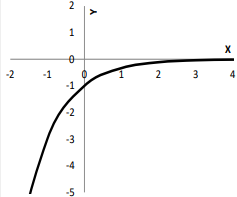
\includegraphics[width=0.45\textwidth]{capitulos/potencias_e_funcoes_exponenciais/media/image11.png} 
    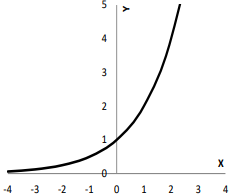
\includegraphics[width=0.45\textwidth]{capitulos/potencias_e_funcoes_exponenciais/media/image12.png}
\end{figure}

\begin{figure}[H]
    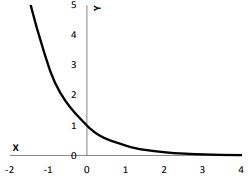
\includegraphics[width=0.45\textwidth]{capitulos/potencias_e_funcoes_exponenciais/media/image13.png} 
    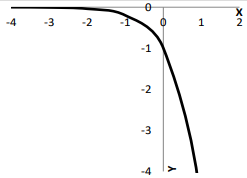
\includegraphics[width=0.45\textwidth]{capitulos/potencias_e_funcoes_exponenciais/media/image14.png}
\end{figure}

\textbf{Solução: }

1º gráfico: letra (c): o sinal de menos na frente de \textit{h(x)} indica que o parâmetro \textit{A = -1}, portanto esta função corta \textit{y} em (\textit{0,-1}) ; é negativa para qualquer \textit{x}eé o rebatimento da função   \textit{y = 3\textsuperscript{ - x}} , que é uma exponencial decrescente (Veja letra (b)).

2º gráfico: letra (a): \textit{A = 1} indica que \textit{f(x)} é positiva. O expoente \textit{m = 1 }(positivo),  indicaque  \textit{f(x)} é crescente. 

3º gráfico: letra (b): \textit{A = 1} indica que \textit{g(x)} é positiva. O expoente \textit{m = -1 }(negativo),  indicaque  \textit{g(x)} é decrescente. 

4º gráfico: letra (d): \textit{A = -1 } indicaque  \textit{p(x)} corta \textit{y} em (\textit{0,-1}) ; é negativa para qualquer \textit{x}eé o rebatimento da função   \textit{y = 5\textsuperscript{ x}} , que é uma exponencial crescente (semelhante a função da letra (a)) \qedsymbol{}
\end{texemplo}

\subsection{Função exponencial com base e (função exponencial natural)}

\begin{caixa}
\textbf{Definição:} A função exponencial natural tem a forma

  \textit{f(x) = A$ \cdot $  e \textsuperscript{m $ \cdot $  x}} (3.1)

onde osparâmetros  \textit{A }e \textit{m} $ \in \mathbb{R} $ e a base \textit{e} é um número irracional, chamado  número de Euler: 2.7182818...
\end{caixa}

\begin{texemplo}
Faça os gráficos das funções \textit{f(x) =  e\textsuperscript{ x}} e  \textit{g(x) =  e\textsuperscript{ - x}} :

\textbf{Solução}: Atribuindo valores para \textit{x}, obtém-se os valores de \textit{f} e \textit{g}. A figura abaixo mostras estas funções, que são semelhantes às exponenciais de base qualquer. 

\begin{figure}[H]
    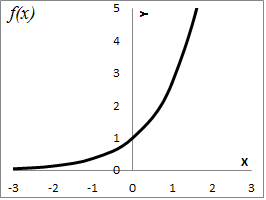
\includegraphics[width=0.45\textwidth]{capitulos/potencias_e_funcoes_exponenciais/media/image15.png} 
    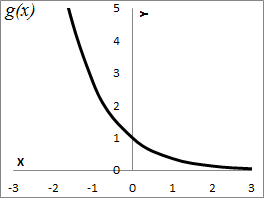
\includegraphics[width=0.45\textwidth]{capitulos/potencias_e_funcoes_exponenciais/media/image16.png}
\end{figure}
\end{texemplo}

\begin{exercicios}
\exitem{} I) Faça e compare os gráficos das funções.  

 a) \textit{f(x) = 3\textsuperscript{x}} e \textit{ f(x) = -3\textsuperscript{x}}

 b) \textit{f(x) = 4\textsuperscript{x}} e \textit{f(x) = -4\textsuperscript{x}}

II) Qual é o efeito do sinal do parâmetro \textit{A} no gráfico das funções \textit{f(x)= Ab\textsuperscript{mx}}?

\exitem{} I) Faça e compare os gráficos das funções. 

  a) \textit{f(x) = 3\textsuperscript{x}}  e \textit{f(x) = 3\textsuperscript{-x  }}
  
  b) \textit{f(x) = -3\textsuperscript{x}}\textsuperscript{ }e  \textit{f(x) = -3\textsuperscript{-x}}

 II) Qual é o efeito do sinal do parâmetro \textit{m} no gráfico das funções \textit{f(x)= Ab\textsuperscript{mx}}?

\exitem{} Faça um esboço do gráfico das funções, com base nas conclusões dos Exercícios 1 e 2.

    a) \textit{f(x) = 5\textsuperscript{x}}
    
    b) \textit{f(x) = -5\textsuperscript{x}}
    
    c) \textit{f(x) = -2\textsuperscript{-x }}
    
    d) \textit{f(x) = -7\textsuperscript{x}}

\exitem{} Faça um esboço do gráfico das funções:

a) f\textit{(x) = 2$ \cdot $ 5\textsuperscript{x}}

b) \textit{f(x) = 3 $ \cdot $  5\textsuperscript{x}}

c) \textit{f(x) = -2 $ \cdot $  2\textsuperscript{-x}}

d) \textit{f(x) = -3 $ \cdot $  7\textsuperscript{x}}

\exitem{} Faça um esboço do gráfico das funções:

a) \textit{f(x) = 2$ \cdot $ 2\textsuperscript{x}}

b) \textit{f(x) = 5\textsuperscript{x+1}}

c) \textit{f(x) = 2\textsuperscript{-x+2}}

d) \textit{f(x) = 7\textsuperscript{x-1}}

\item Faça os gráficos do exercício anterior usando um aplicativo computacional.

\exitem{} Faça os gráficos das funções:

a) \textit{f(x) = e\textsuperscript{2x}}

b) \textit{f(x) = -e\textsuperscript{-2x  }}

c) \textit{f(x) = 3e\textsuperscript{x}}

d) \textit{f(x) = -2e\textsuperscript{-3x}}

\item Faça os gráficos do exercício anterior usando um aplicativo computacional.

\exitem{} Associe as funções 

a) \textit{f(x) = 2$ \cdot $ e\textsuperscript{x}};

(b) \textit{g(x) = 2$ \cdot $ 3\textsuperscript{-x}};

(c) \textit{h(x) = -2$ \cdot $ 3\textsuperscript{-x}};

(d) \textit{p(x) = -2$ \cdot $ 5 \textsuperscript{x}}

aos respectivos gráficos. (Justifique sua resposta)

\begin{figure}[H]
    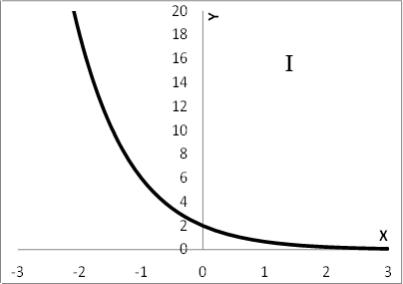
\includegraphics[width=0.45\textwidth]{capitulos/potencias_e_funcoes_exponenciais/media/image17.png} 
    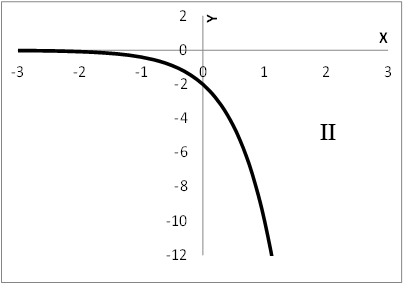
\includegraphics[width=0.45\textwidth]{capitulos/potencias_e_funcoes_exponenciais/media/image18.png}
\end{figure}

\begin{figure}[H]
    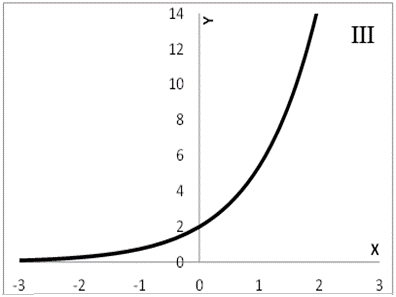
\includegraphics[width=0.45\textwidth]{capitulos/potencias_e_funcoes_exponenciais/media/image19.png} 
    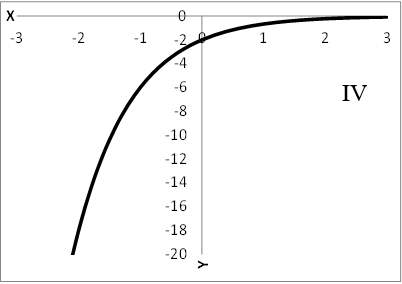
\includegraphics[width=0.45\textwidth]{capitulos/potencias_e_funcoes_exponenciais/media/image20.png}
\end{figure}

\exitem{} Uma aplicação a juros compostos (juro sobre juro) evolui com taxa mensal de 10$\%$  ao mês, de acordo com a tabela abaixo. Elabore uma função exponencial para calcular o montante depois de 25 meses. 

\begin{table}[H]
 			\centering
\begin{tabular}{p{1.08in}p{0.88in}}
\hline
%row no:1
\multicolumn{1}{|p{1.08in}}{Tempo (meses)} & 
\multicolumn{1}{|p{0.88in}|}{Capital (R$\$$ )} \\
\hhline{--}
%row no:2
\multicolumn{1}{|p{1.08in}}{0} & 
\multicolumn{1}{|p{0.88in}|}{1.000,00} \\
\hhline{--}
%row no:3
\multicolumn{1}{|p{1.08in}}{1} & 
\multicolumn{1}{|p{0.88in}|}{1.100,00} \\
\hhline{--}
%row no:4
\multicolumn{1}{|p{1.08in}}{2} & 
\multicolumn{1}{|p{0.88in}|}{1.210,00} \\
\hhline{--}
%row no:5
\multicolumn{1}{|p{1.08in}}{3} & 
\multicolumn{1}{|p{0.88in}|}{1.331,00} \\
\hhline{--}
%row no:6
\multicolumn{1}{|p{1.08in}}{...} & 
\multicolumn{1}{|p{0.88in}|}{...} \\
\hhline{--}

\end{tabular}
 \end{table}
\end{exercicios}

\section{Juros compostos}

Em uma aplicação financeira do tipo poupança, o capital inicial \textit{C\textsubscript{o }}é depositado no mês \textit{t = 0} e é corrigido mensalmente com uma taxa de juros constante de \textit{i $\%$ } do capital presente. O capital a cada mês pode ser calculado da seguinte maneira:

Capital = Capital do mês anterior + rendimento

Onde o rendimento é : Capital do mês anterior \textit{ $ \cdot $  } taxa de juros.

\begin{table}[H]
 			\centering
\begin{tabular}{p{0.59in}p{1.77in}p{1.08in}}
\hline
%row no:1
\multicolumn{1}{|p{0.59in}}{Tempo (meses)} & 
\multicolumn{1}{|p{1.77in}}{Capital (R$\$$ )} & 
\multicolumn{1}{|p{1.08in}|}{Montante (R$\$$ )} \\
\hhline{---}
%row no:2
\multicolumn{1}{|p{0.59in}}{0} & 
\multicolumn{1}{|p{1.77in}}{\textit{C\textsubscript{o}}} & 
\multicolumn{1}{|p{1.08in}|}{\textit{C\textsubscript{o}}} \\
\hhline{---}
%row no:3
\multicolumn{1}{|p{0.59in}}{1} & 
\multicolumn{1}{|p{1.77in}}{\textit{C\textsubscript{o}+ C\textsubscript{o} $ \cdot $  i/100 }} & 
\multicolumn{1}{|p{1.08in}|}{\textit{C\textsubscript{o} $ \cdot $  (1+i/100)}} \\
\hhline{---}
%row no:4
\multicolumn{1}{|p{0.59in}}{2} & 
\multicolumn{1}{|p{1.77in}}{\textit{C\textsubscript{o} $ \cdot $  (1+i/100) $ \cdot $  (1+i/100)}} & 
\multicolumn{1}{|p{1.08in}|}{\textit{C\textsubscript{o} $ \cdot $  (1+i/100)\textsuperscript{2}}} \\
\hhline{---}
%row no:5
\multicolumn{1}{|p{0.59in}}{3} & 
\multicolumn{1}{|p{1.77in}}{\textit{C\textsubscript{o} $ \cdot $  (1+i/100)\textsuperscript{2}} \textit{$ \cdot $  (1+i/100)} } & 
\multicolumn{1}{|p{1.08in}|}{\textit{C\textsubscript{o} $ \cdot $  (1+i/100)\textsuperscript{3}}} \\
\hhline{---}
%row no:6
\multicolumn{1}{|p{0.59in}}{4} & 
\multicolumn{1}{|p{1.77in}}{\textit{C\textsubscript{o} $ \cdot $  (1+i/100)\textsuperscript{3} $ \cdot $  (1+i/100)} } & 
\multicolumn{1}{|p{1.08in}|}{\textit{C\textsubscript{o} $ \cdot $  (1+i/100)\textsuperscript{4}}} \\
\hhline{---}
%row no:7
\multicolumn{1}{|p{0.59in}}{...} & 
\multicolumn{1}{|p{1.77in}}{...} & 
\multicolumn{1}{|p{1.08in}|}{....} \\
\hhline{---}
%row no:8
\multicolumn{1}{|p{0.59in}}{\textit{t}} & 
\multicolumn{1}{|p{1.77in}}{\textit{C\textsubscript{o} $ \cdot $  (1+i/100)\textsuperscript{t-1}$ \cdot $  (1+i/100)} } & 
\multicolumn{1}{|p{1.08in}|}{\textit{C\textsubscript{o} $ \cdot $  (1+i/100)\textsuperscript{t}}} \\
\hhline{---}

\end{tabular}
 \end{table}

Generalizando, para \textit{t} meses, o montante será

 \( C \left( t \right) =C_{0} \left( 1+\frac{i}{100} \right) ^{t} \)       (4.1)

\begin{texemplo}
Uma poupança foi iniciada com R$\$$  5.000,00 e corrigida com uma taxa constante de 0,6 $\%$  ao mês. Calcule o montante depois de (a) 15 meses (b) 10 anos.

\textbf{Solução}: (a) aplicando \textit{t = 15} meses e \textit{C\textsubscript{o} = 5.000,00} na Eq. 4.1, tem-se:

 \[  \]  \[ C \left( 15 \right) =5000 \left( 1+\frac{0,6}{100} \right) ^{15} \] 

  \( C \left( 15 \right) =5.469,40  \)  reais.

(b) Fazendo \textit{t = 10 $ \cdot $  12 = 120} meses e substituindo na Eq. 4.1, tem-se:

 \[  \]  \[ C \left( 120 \right) =5000 \left( 1+\frac{0,6}{100} \right) ^{120} \] 

  \( C \left( 120 \right) =10.250,09  \) reais \qedsymbol{}
\end{texemplo}

\begin{exercicios}
\exitem{} Dados o capital inicial, a taxa de juros e o tempo, calcule o montante de aplicações a juros compostos:

\begin{enumerate}[label=\alph*)]
	\item \textit{C\textsubscript{o }} \textit{= R$\$$  1.500,00} ,  \textit{i = 0,5 }$\%$  ao mês e  \textit{t = 20} meses

	\item \textit{C\textsubscript{o }} \textit{= R$\$$  10.000,00} , \textit{i = 1 }$\%$ ao mês  e  \textit{t = 50 }meses.

	\item \textit{C\textsubscript{o }} \textit{= R$\$$  10.500,00} , \textit{i = 1 }$\%$ ao mês  e  \textit{t = 5 }anos.

	\item \textit{C\textsubscript{o }} \textit{= R$\$$  1.000,00} , \textit{i = 0,8 }$\%$ ao mês  e  \textit{t = 10 }anos e\textit{ 5 }meses.

	\item \textit{C\textsubscript{o }} \textit{= R$\$$  20.000,00} , \textit{i = 0,65 }$\%$ ao mês  e  \textit{t = 3 }anos e 10 meses.
\end{enumerate}

\exitem{} Qual é o capital inicial de uma aplicação com taxa \textit{i = 0,5 }$\%$  ao mês, cujo montante depois de 10 anos é de R$\$$  8.500,00.

\exitem{} Faça os gráficos das seguintes aplicações com \textit{C\textsubscript{o }} \textit{= R$\$$  10.000,00},  \textit{i = 2 }$\%$ ao mês  para tempo de 0 a \textit{\colorbox{yellow}{12}}\colorbox{yellow}{ meses:} 

a) Corrigidos com \colorbox{yellow}{juros simples}

b) Corrigidos com juros compostos.

\exitem{} Verifique quando as aplicações abaixo terão o mesmo montante:

a)  \textit{C\textsubscript{o }} \textit{= R$\$$  12.000,00},  \textit{i = 1 }$\%$  ao mês, corrigidos com juros simples.

b) \textit{C\textsubscript{o }} \textit{= R$\$$  10.000,00},  \textit{i = 1 }$\%$  ao mês, corrigidos com juros compostos.

\exitem{} Qual é o capital inicial para que o montante de uma aplicação seja R$\$$  20.000,00, depois de 3 anos, com taxa de 1 $\%$  ao mês?

\exitem{} Um pai emprestou R$\$$  5.000,00 ao filho, a 1$\%$  ao mês, a juros compostos. Qual é a dívida depois de 1 ano.

\exitem{} Um investidor tem R$\$$  250.000,00 para comprar um apartamento, que deverá ser entregue em 1 ano. Foram-lhe oferecidas três formas de pagamento. Verifique qual delas é a mais vantajosa para ele, considerando que o capital pode ser aplicado (se não for usado para pagar) com taxa de 0,6 $\%$  ao mês:

a) À vista R$\$$  240.000,00.

b) Entrada R$\$$  100.000,00 e R$\$$  150.000,00 na entrega do apartamento.

c) R$\$$  260.000,00 na entrega do apartamento.

\exitem{} Calcule a taxa de juros na venda de uma máquina agrícola, cujo preço à vista é R$\$$  20.000,00 e para pagar em 6 meses é R$\$$ 22.000,00.  
\end{exercicios}

\section{RESPOSTAS DOS EXERCÍCIOS PROPOSTOS}

\begin{respostas}{2}
	\ansitem{} a) 16 \\ b) -64 \\ c) 0 \\ d) 1 \\ e) 1/8 \\  f) 9/16 \\ g) 16/81 \\ h) -625

	\ansitem{} a) 64 \\ b) 1/1024 \\ c) 9 \\ d) 729/64 \\ e) 5/4 \\ f) 1/125 \\  g) 16/49 \\ h) 512

    \ansitem{} a) 1/8 \\ b) 1/243 \\ c) 64/27 \\ d) 16/9
    
    \setcounter{enumi}{5}

	\ansitem{} a) 32/25 \\ b) -16/3 \\  c) 8 \\  d) 504 \\  e) 9/32 \\  f) -78125/1944

	\ansitem{} a) 3/5 \\ b) 1/49 \\  c) 2 \\  d) 1

	\ansitem{} a) x = 3 \\ b) x = 3/2 \\ c)x = -3/2 \\ d) x = 1 \\ e) x = -2/5 \\ f) x = 1.

    \ansitem{} x\textsubscript{1 }= -1 e x\textsubscript{2} = -8.
\end{respostas}

\begin{respostas}{3}
	\ansitem{} (I) a) \tab b)

\begin{figure}[H]
    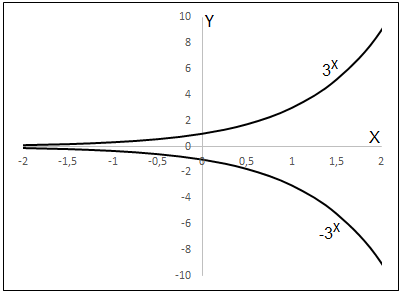
\includegraphics[width=0.45\textwidth]{capitulos/potencias_e_funcoes_exponenciais/media/image21.png} 
    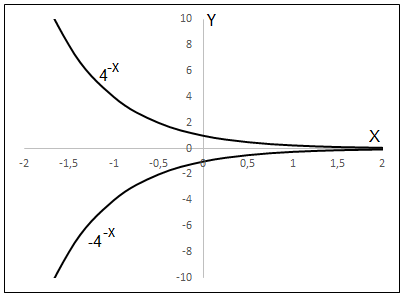
\includegraphics[width=0.45\textwidth]{capitulos/potencias_e_funcoes_exponenciais/media/image22.png}
\end{figure}

II- Se \textit{A} for positivo a função é positiva e se \textit{A} for negativo a função é negativa. As funções \textit{f(x)=Ab\textsuperscript{x}} e \textit{g(x)=-Ab\textsuperscript{x}} são simétricas em relação ao eixo X.

\ansitem{}  (I)a \tab b

\begin{figure}[H]
    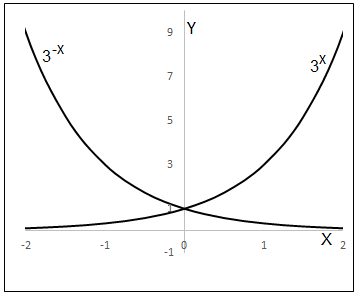
\includegraphics[width=0.45\textwidth]{capitulos/potencias_e_funcoes_exponenciais/media/image23.png} 
    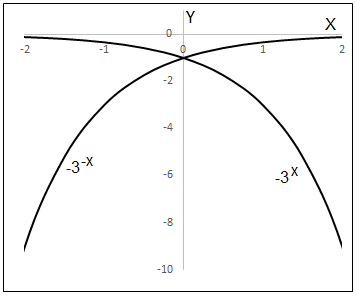
\includegraphics[width=0.45\textwidth]{capitulos/potencias_e_funcoes_exponenciais/media/image24.png}
\end{figure}

II- Se \textit{f(x)=Ae\textsuperscript{mx}} e \textit{g(x)=Ae\textsuperscript{-mx}} então \textit{f} e \textit{g} são simétricas em relação ao eixo Y.

\ansitem{} a) \tab b)

\begin{figure}[H]
    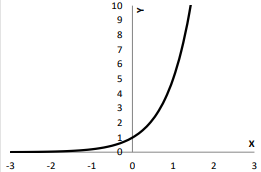
\includegraphics[width=0.45\textwidth]{capitulos/potencias_e_funcoes_exponenciais/media/image25.png} 
    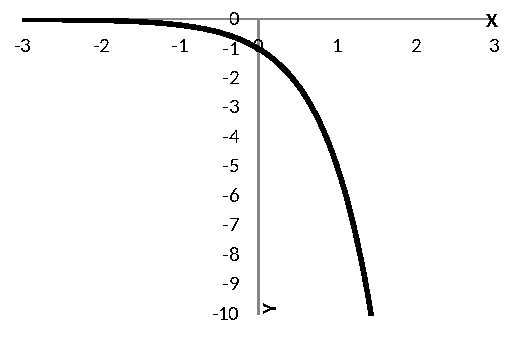
\includegraphics[width=0.45\textwidth]{capitulos/potencias_e_funcoes_exponenciais/media/image26.pdf}
\end{figure}

c) \tab d)

\begin{figure}[H]
    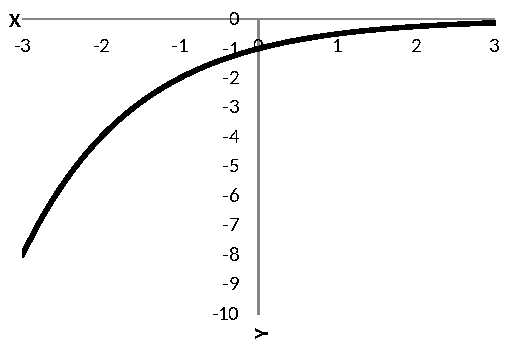
\includegraphics[width=0.45\textwidth]{capitulos/potencias_e_funcoes_exponenciais/media/image27.pdf} 
    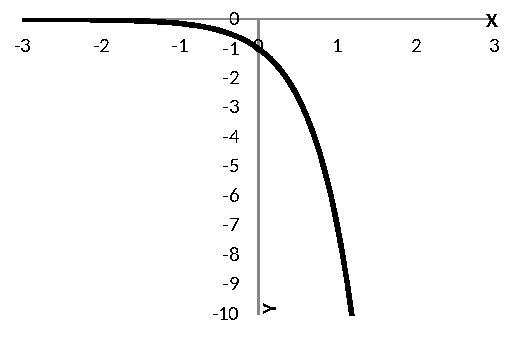
\includegraphics[width=0.45\textwidth]{capitulos/potencias_e_funcoes_exponenciais/media/image28.pdf}
\end{figure}

\ansitem{} a) \tab b)

\begin{figure}[H]
    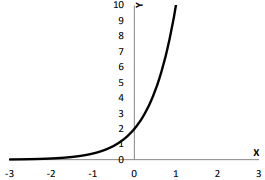
\includegraphics[width=0.45\textwidth]{capitulos/potencias_e_funcoes_exponenciais/media/image29.png} 
    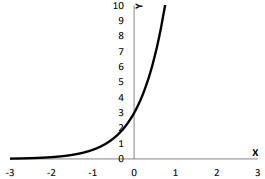
\includegraphics[width=0.45\textwidth]{capitulos/potencias_e_funcoes_exponenciais/media/image30.png}
\end{figure}

c) \tab d)

\begin{figure}[H]
    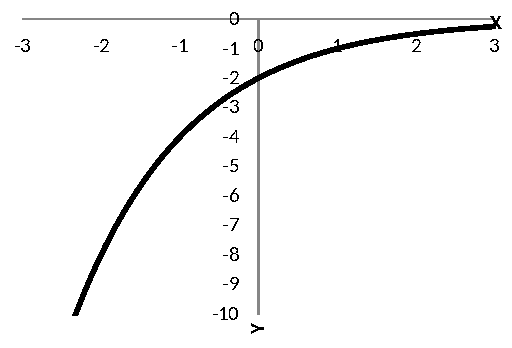
\includegraphics[width=0.45\textwidth]{capitulos/potencias_e_funcoes_exponenciais/media/image31.pdf} 
    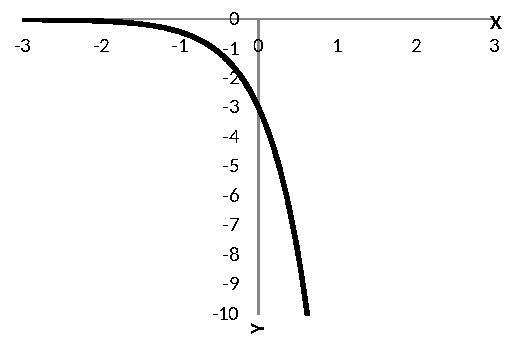
\includegraphics[width=0.45\textwidth]{capitulos/potencias_e_funcoes_exponenciais/media/image32.pdf}
\end{figure}

\ansitem{} a) \tab b)

\begin{figure}[H]
    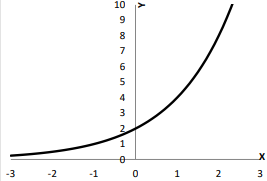
\includegraphics[width=0.45\textwidth]{capitulos/potencias_e_funcoes_exponenciais/media/image33.png} 
    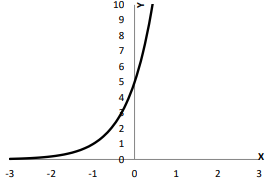
\includegraphics[width=0.45\textwidth]{capitulos/potencias_e_funcoes_exponenciais/media/image34.png}
\end{figure}

c) \tab d)

\begin{figure}[H]
    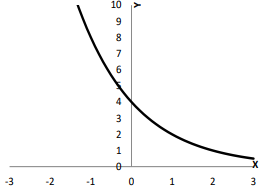
\includegraphics[width=0.45\textwidth]{capitulos/potencias_e_funcoes_exponenciais/media/image35.png} 
    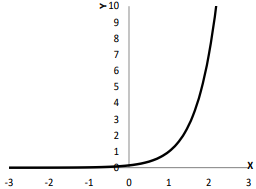
\includegraphics[width=0.45\textwidth]{capitulos/potencias_e_funcoes_exponenciais/media/image36.png}
\end{figure}

    \stepcounter{enumi}

	\ansitem{} a) \tab b)

\begin{figure}[H]
    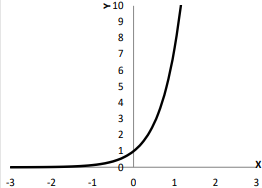
\includegraphics[width=0.45\textwidth]{capitulos/potencias_e_funcoes_exponenciais/media/image37.png} 
    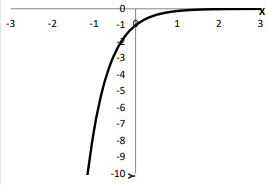
\includegraphics[width=0.45\textwidth]{capitulos/potencias_e_funcoes_exponenciais/media/image38.png}
\end{figure}

    c) \tab d)

\begin{figure}[H]
    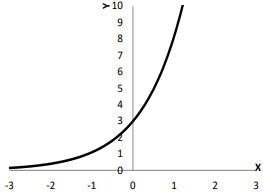
\includegraphics[width=0.45\textwidth]{capitulos/potencias_e_funcoes_exponenciais/media/image39.png} 
    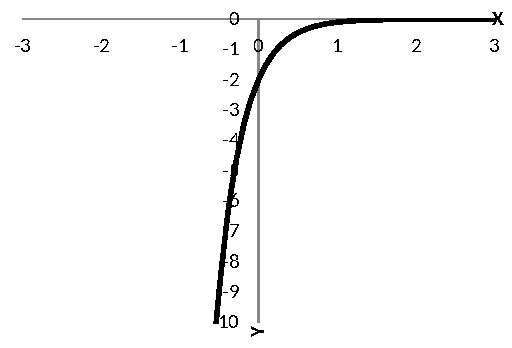
\includegraphics[width=0.45\textwidth]{capitulos/potencias_e_funcoes_exponenciais/media/image40.pdf}
\end{figure}

    \stepcounter{enumi}

    \ansitem{} a-III ; b-I;c-IV;  d-II . 

	\ansitem{} \( C \left( t \right) =C_{0} \left( 1+\frac{i}{100} \right) ^{t} \)
\end{respostas}

\begin{respostas}{4}
\ansitem{} a) \textit{R$\$$  1 657,34}

 b) \textit{R$\$$  16 446,32}

 c) \textit{R$\$$  19 075,32}

 d) \textit{R$\$$  2 707,49}

 e) \textit{R$\$$  26 944,11}

\ansitem{} \( C_{o} \cong  R\$ 4 671,88 \) 

\begin{figure}[H]
    \ansitem{}

	\begin{Center}
		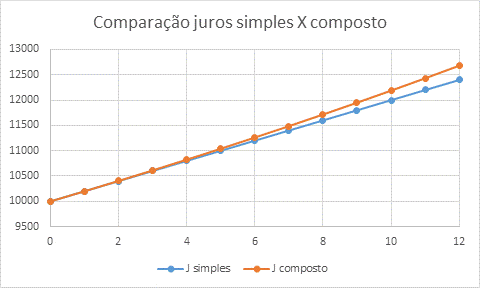
\includegraphics[width=3.23in,height=2.2in]{capitulos/potencias_e_funcoes_exponenciais/media/image41.png}
	\end{Center}
\end{figure}

\ansitem{} Tempo no qual as duas aplicações são iguais = 74º mês.

Sugestão: desenvolva as duas aplicações em uma tabela eletrônica.

\begin{figure}[H]
	\begin{Center}
		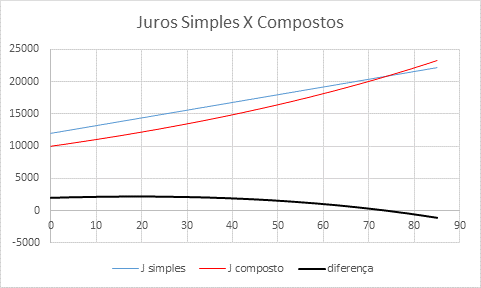
\includegraphics[width=3.62in,height=2.18in]{capitulos/potencias_e_funcoes_exponenciais/media/image42.png}
	\end{Center}
\end{figure}

\ansitem{}  \( C_{o} \cong  R\$ 13 978,50 \) 

\ansitem{} \textit{R$\$$  5 634,13}

\ansitem{} Alternativa b.

\ansitem{}  \( i \cong 1,6 \) 01
\end{respostas}